%Copyright 2014 Jean-Philippe Eisenbarth
%This program is free software: you can 
%redistribute it and/or modify it under the terms of the GNU General Public 
%License as published by the Free Software Foundation, either version 3 of the 
%License, or (at your option) any later version.
%This program is distributed in the hope that it will be useful,but WITHOUT ANY 
%WARRANTY; without even the implied warranty of MERCHANTABILITY or FITNESS FOR A 
%PARTICULAR PURPOSE. See the GNU General Public License for more details.
%You should have received a copy of the GNU General Public License along with 
%this program.  If not, see <http://www.gnu.org/licenses/>.

%Based on the code of Yiannis Lazarides
%http://tex.stackexchange.com/questions/42602/software-requirements-specification-with-latex
%http://tex.stackexchange.com/users/963/yiannis-lazarides
%Also based on the template of Karl E. Wiegers
%http://www.se.rit.edu/~emad/teaching/slides/srs_template_sep14.pdf
%http://karlwiegers.com
\documentclass{scrreprt}
\usepackage{listings}
\usepackage{underscore}
\usepackage[bookmarks=true]{hyperref}
\usepackage[utf8]{inputenc}
\usepackage[english]{babel}
\usepackage{color}
\usepackage{graphicx}
\graphicspath{ {images/} }

\definecolor{dkgreen}{rgb}{0,0.6,0}
\definecolor{gray}{rgb}{0.5,0.5,0.5}
\definecolor{mauve}{rgb}{0.58,0,0.82}

\lstset{frame=tb,
  language=Java,
  aboveskip=3mm,
  belowskip=3mm,
  showstringspaces=false,
  columns=flexible,
  basicstyle={\small\ttfamily},
  numbers=none,
  numberstyle=\tiny\color{gray},
  keywordstyle=\color{blue},
  commentstyle=\color{dkgreen},
  stringstyle=\color{mauve},
  breaklines=true,
  breakatwhitespace=true,
  tabsize=3
}
\hypersetup{
    bookmarks=false,    % show bookmarks bar?
    pdftitle={SmartGlove BLE API User's Guide},    % title
    pdfauthor={Matthew Constant},                     % author
    pdfsubject={SmartGlove Application Development},                        % subject of the document
    pdfkeywords={SmartGlove, API, Android}, % list of keywords
    colorlinks=true,       % false: boxed links; true: colored links
    linkcolor=blue,       % color of internal links
    citecolor=black,       % color of links to bibliography
    filecolor=black,        % color of file links
    urlcolor=purple,        % color of external links
    linktoc=page            % only page is linked
}%
\def\myversion{1.0 }
\date{}
%\title
\usepackage{hyperref}
\begin{document}

\begin{flushright}
    \rule{16cm}{5pt}\vskip1cm
    \begin{bfseries}
        \Huge{User's Guide}\\
        \vspace{1.9cm}
        for\\
        \vspace{1.9cm}
        SmartGlove BLE API\\
        \vspace{1.9cm}
        \LARGE{Version \myversion}\\
        \vspace{1.9cm}
        Prepared by Matthew Constant\\
        \vspace{1.9cm}
       Wearable Biosensing Lab\\
        \vspace{1.9cm}
        \today\\
    \end{bfseries}
\end{flushright}

\tableofcontents


%\chapter*{Revision History}

%\begin{center}
    %\begin{tabular}{|c|c|c|c|}
        %\hline
	 %   Name & Date & Reason For Changes & Version\\
        %\hline
	 %   21 & 22 & 23 & 24\\
%        \hline
%	    31 & 32 & 33 & 34\\
    %    \hline
   % \end{tabular}
%\end{center}

\chapter{API Overview}

\section{Background}
The SmartGlove BLE API was developed for Android mobile devices (smartphones, tablets).
If you are not familar with Android application development, this section will give background 
on relevent aspects needed in this document. Otherwise, you can skip this section and
go straight to \textit{SmartGlove Bluetooth Models}.\\
Android applications consists of three basic components: Activities, Services, and Broadcast Receivers.
Activities are the graphical part of the application which the User interacts with directly.
Activities deal with event driven operations such as when a button is clicked or when to 
display information (for example, to show a picture once is has been downloaded.
An activity is the only component that the User will interact with. Services run in the
background and are usually designed to complete a single specific task. The most common
example to demostrate the difference between an activity and a service is a music streaming
application. The activity will dislay the song being played and allow the User to pause, play, etc.
One possible service in this case would be a service to download the song information (another
would be a service to play the audio). The last component, Broadcast Receivers, are meant to
allow separate processes, components, or applications to communicate useful information, i.e. battery percentage.
Usually, data that is boradcast is not specific to any one application but could be useful to many
different applications serving many different purposes. Services and activities can both send
and receive broadcasts by implementing or registering a broadcast receiver. Broadcast 
receivers can also be implemented as a stand-alone component, however this is not relevent
to the SmartGlove API.\\
In order for all of these different components to interact, some kind of \''messenger\'' is
needed. In Android, this messenger is called an Intent. A component (described above)
will create an Intent and send it to the component it wants to start, stop or communicate with.
The Intent can also contain extra information called \''Extras\''. These extras can be
Strings, ints, floats, or (most importantly in this case) serializable objects. Calling applications 
interact with the SmartGlove by sending Intents filled with specific information. Luckily, BluetoothLeService
provides static methods to take care of packaging the Intents so the Caller does not need to worry
about this.

\section{SmartGlove Bluetooth Models and the Manager}
The most fundamental aspect of the SmartGlove BLE API is the BluetoothLeModel. This class is
used to represent generic BLE devices. It contains the device address, its current connection
state, and a list of its services (represented by BluetoothServiceModels). BluetoothServiceModels
contain the service's UUID as well as a list of all of its characteristics (represented by
BluetoothCharacteristicModels). BluetoothCharacteristicModels contains the characteristic's
UUID as well as its current value as a byte[]. By using these models, an abstraction layer is created
between the actual BLE device and the API, simplfying the process of communicating with the 
BLE device.
\begin{lstlisting}
// BluetoothLeModelManager
BluetoothLeModel CREATE(String BD_ADDR);
BluetoothLeModel GET(String BD_ADDR);

// BluetoothLeModel
BleStatus getStatus();
void setStatus(BleStatus);
String getAddress();
List<BluetoothServiceModel> getServices();
void setServices(List<BluetoothGattService>);

// BluetoothServiceModel
UUID getUuid();
BluetoothCharacteristicModel getCharacteristics();

// BluetoothCharacteristicModel
UUID getUuid();
byte[] getValue();
void setValue(byte[]);
\end{lstlisting}

\section{BluetoothLeService}
The BluetoothLeService is the main service provided by the SmartGlove
BLE API. This service provides actions to allow the caller to interact with
a BLE device as well as updates to allow the Caller to receive information
related to a connected BLE device. Every action that is supported by this
service is made available by a static method. The general syntax for
an action call is \begin{verbatim}BluetoothLeService.action(Context, BluetoothLeModel)\end{verbatim}
where the BluetoothLeModel is retrieved from BluetoothLeModelManager.
If the caller is expecting to receive information back from the action requested,
it must implement a BleUpdateReceiver, and wait for the appropriate update
to be broadcast to the receiver (this is covered in more detail in the next section).
Current actions supported by this service are:\\
\begin{itemize}
	\item{START - Start the Service and allow it to run in the background.}
	\item{STOP - Stop the Service if running. This causes all connected devices
	to be disconnected.}
\end{itemize}


\section{BleUpdateReceiver}
The BleUpdateReceiver is a Broadcast Receiver used to transmit \''Update Packets\'' to
all listening components (activities or services). An update packet consists of
the BleUpdate, such as UPDATE_CONNECTED, and the BluetoothLeModel which
represents the BLE device corresponding to the update. In order for a component
to implement the BleUpdateReceiver and begin listening for updates, it must do two things.
First, it must create an inner class which extends the BleUpdateReceiver abstract class.
This is the receiver which will receive the updates. Usually, a switch statement is used inside the
onReceive() method for each possible update. The second thing that must be done is to register
this receiver, preferably in the onStart() method, and unregister the receiver, preferably in the
onStop() method. An example setup is shown below.
\pagebreak
\begin{lstlisting}
@Override
public void onStart() {
	super.onStart();
	this.registerReceiver(mBleUpdateReceiver, BleUpdateReceiver.INTENT_FILTER);
	...
}

@Override
public void onStop() {
	this.unregisterReceiver(mBleUpdateReceiver);
	...
	super.onStop();
}

private BleUpdateReceiver mBleUpdateReceiver = new BleUpdateReceiver() {
        @Override
        public void onReceive(Context context, Intent intent) {
            int update = intent.getIntExtra(BleUpdateReceiver.EXTRA_UPDATE, -1);
            switch(update) {
                case BleUpdateReceiver.UPDATE_CONNECTED:
                    // May want to call BleConnectionService.DISCOVER_SERVICES(mContext, mBluetoothLeModel) here
                    break;
                case BleUpdateReceiver.UPDATE_DISCONNECTED:

                    break;
                case BleUpdateReceiver.UPDATE_SERVICES_DISCOVERED:
                   
                    break;
                 ...
                default:

                    break;
            }
        }
};
\end{lstlisting}


\chapter{Interacting with SmartGlove via BluetoothLeService}
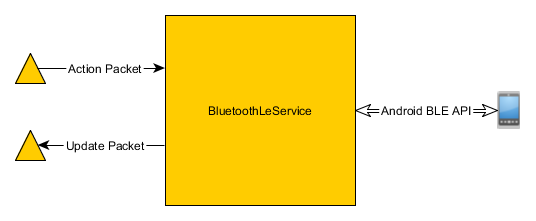
\includegraphics[width=\textwidth]{BluetoothLeServiceOverview}

\section{Action Packets}
Action packets are sent using Intents. In general, they are composed
the following way:
\begin{lstlisting}
Intent intent = new Intent(context, BluetoothLeService.class);
intent.putExtra(EXTRA_ACTION, BleAction.<Action>.getAction());	// Set BleAction
intent.putExtra(EXTRA_DEVICE, bluetoothLeModel);			// Set BluetoothLeModel
\end{lstlisting}
This packet is then sent to BluetoothLeService via the following call:
\begin{verbatim}context.startService(intent);\end{verbatim}
This packaging is taken care of by the BluetoothLeService itself,
allowing the caller to simply call a static method to send an action
to the BluetoothLeService. For example, the following snippet
sends the START action to BluetoothLeService:
\begin{verbatim}BluetoothLeService.START(context);\end{verbatim}

\section{Update Packets}
Update packets are transmitted using Intents, similar to Action packets.
When a BleUpdateReceiver receives a broadcast, the intent will contain
an int representing the BleUpdate and a BluetoothLeModel corresponding
to the relevent BLE device. One thing to note is that when a device is 
connected to, the BluetoothLeModel's service list is either empty or
out of date. In order to interact with the device's services and characteristics,
the caller must first send the DISCOVER_SERVICES actions when an already
connected BluetoothLeModel. Typically, this is done when the UPDATE_CONNECTED
update packet is received.


\chapter{Contributing to SmartGlove BLE API}

\section{Adding Actions}
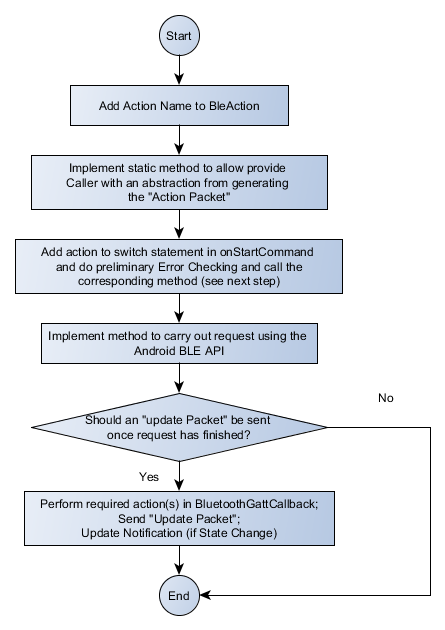
\includegraphics[width=\textwidth]{AddActionFlowchart}

\section{Sending Updates}
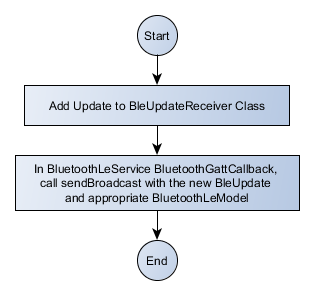
\includegraphics[width=\textwidth]{AddUpdateFlowchart}



\end{document}